\section{支持向量机}
现阶段,我们假设训练数据集在特征空间中是线性可分的,即根据定义,存在至少一个参数$\boldsymbol{w}$和$b$的选择方式,使得对于$t_n=+1$的点,$y(\boldsymbol{x}_n)>0$,对于$t_n=-1$的点,都有$y(\boldsymbol{x}_n)<0$,从而对于所有训练数据点,都有$t_ny(\boldsymbol{x}_n)>0$。

当然,存在许多能够把类别精确分开的解。我们介绍过感知器算法,它能够保证在有限步骤之内找到一个解。然而,它找到的这个解依赖于$\boldsymbol{w}$和$b$的(任意的)初始值选择,还依赖于数据点出现的顺序。如果有多个能够精确分类训练数据点的解,那么我们应该尝试寻找泛化错误最小的那个解。支持向量机解决这个问题的方法是:引入边缘(margin)的概念,这个概念被定义为决策边界与任意样本之间的最小距离。

在支持向量机中,决策边界被选为使边缘最大化的那个决策边界。采用最大边缘解的动机可以通过计算学习理论或者统计学习理论进行理解。对于一个简单的线性可分数据集,在贝叶斯方法中,关于参数的先验概率分布进行积分或求和,可以产生一个决策边界,这个决策边界位于分开数据点的区域中间。最大边缘解有着类似的行为。

对偶问题使得模型能够用核函数重新表示,因此最大边缘分类器可以被高效地应用于维数超过数据点个数的特征空间,包括无穷维特征空间。为了使用训练过的模型分类新的数据点,$y(\boldsymbol{x})$可以根据参数$\{a_n \}$和核函数表示,即
\begin{equation}
\label{713}
	y(\boldsymbol{x})=\sum_{n=1}^{N}a_nt_nk(\boldsymbol{x},\boldsymbol{x}_n)+b
\end{equation}
这种形式的限制的最优化问题满足KKT条件。在这个问题中,下面三个性质要成立 
\begin{flalign}
	a_n\geqslant 0\\
	t_ny(\boldsymbol{x})-1 \geqslant 0\\
	a_n\{t_ny(\boldsymbol{x})-1 \}=0
\end{flalign}
因此对于每个数据点,要么$a_n=0$,要么$t_ny(\boldsymbol{x}_n)=1$。任何使得$a_n=0$的数据点都不会出现在公式的求和式中,因此对新数据点的预测没有作用。剩下的数据点被称为支持向量。这个性质是支持向量机在实际应用中的核心。一旦模型被训练完毕,相当多的数据点都可以被丢弃,只有支持向量被保留。说明了SVM稀疏性的来源。

解决了二次规划问题,找到了$\boldsymbol{a}$的值之后,注意到支持向量$\boldsymbol{x}_n$满足$t_ny(\boldsymbol{x}_n=1$,我们就可以确定阈值参数$b$的值。使用公式$\ref{713}$,可得
\begin{equation}
	t_n\left(\sum_{m\in S}a_mt_mk(\boldsymbol{x}_n,\boldsymbol{x}_m)+b \right)=1
\end{equation}
其中$S$表示支持向量的下标集合。通过下面的方式得到一个在数值计算上更加稳定的解。
\begin{equation}
	b=\frac{1}{N_S}\sum_{m\in S}\left(t_n-\sum_{m\in S}a_mt_mk(\boldsymbol{x}_n,\boldsymbol{x}_m) \right)
\end{equation}
其中$N_S$是支持向量的总数。
\subsection*{间隔与支持向量}
给定训练样本集$D=\{(x_1,y_1),\dots,(x_m,y_m)\},y_i\in \{-1,+1\}$,分类学习最基本的想法是基于训练集D在样本空间中找到一个划分超平面,将不同类别的样本分开。如图$\ref{fig:1}$
\begin{figure}
	\centering
	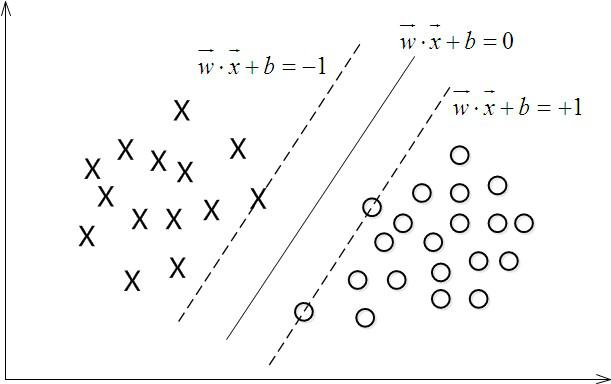
\includegraphics[width=0.7\linewidth]{chapter/统计机器学习/支持向量机/1}
	\caption{}
	\label{fig:1}
\end{figure}

样本空间中任意点$\boldsymbol{x}$到超平面$(\boldsymbol{w},b)$的距离可写为
$$\gamma = \frac{y(w^T x + b)}{\lVert w\rVert} = \frac{yf(x)}{\lVert w \rVert}$$

注:$yf(x)$相当于$\lvert f(x) \rvert$。

假设超平面$(\boldsymbol{w},b)$能将训练样本正确分类,即对于$(x_i,y_i)\in D$,若$y_i=+1,$则有$\boldsymbol{w}^Tx_i+b>0$;若$y_i=-1$,则有$\boldsymbol{w}^Tx_i+b<0$。令
\begin{equation}
\label{eq:1}
\begin{cases} 
\boldsymbol{w}^Tx_i+b\geq +1,\quad y_i=+1;\\
\boldsymbol{w}^Tx_i+b\leq -1,\quad y_i=-1.
\end{cases}
\end{equation}

距离超平面最近的这几个训练样本点使式$\ref{eq:1}$的等号成立,它们被称为“\textbf{支持向量}(support vector)”,两个异类支持向量到超平面的距离之和为
\begin{equation}
\label{eq:2}
\gamma = \frac{2}{\lVert w \rVert},
\end{equation}
它被称为“\textbf{间隔}”(margin)。

欲找到具有“最大间隔”的划分超平面,也就是要找到能满足式$\ref{eq:1}$中约束的参数$\boldsymbol{w}$和$b$,使得$\gamma$最大,即
\begin{equation}
\label{eq:3}
\begin{aligned}
min \quad &\frac{1}{2}\lVert w \rVert^2, \\
s.t. \quad & y_i (w^Tx _i + b) \geq 1, \quad i = 1,\dots, m.
\end{aligned}
\end{equation}
这就是支持向量机的基本型。


\subsection*{对偶问题}
注意到式$\ref{eq:3}$本身是一个凸二次规划问题,能直接用现成的优化计算包求解,但我们可以有更高效的办法。由于这个问题的特殊结构,还可以通过拉格朗日对偶性变换到对偶变量的优化问题,即通过求解与原问题等价的对偶问题得到原始问题的最优解,这就是线性可分条件下支持向量机的对偶算法,这样做的优点在于:
\begin{enumerate}
	\item 对偶问题往往更容易求解;
	\item 可以自然的引入核函数,进而推广到非线性分类问题。	
\end{enumerate}
该问题的拉格朗日函数可写为
\begin{equation}
L(w,b,a) = \frac{1}{2}\lVert w \rVert^2 - \sum_{i=1}^na_i (y_i(w^T x_i + b) - 1)
\end{equation}
然后令
\begin{equation}
\theta (\boldsymbol{w}) = \mathop{\mathrm{max}} \limits_{a_i \geq 0}\ L(\boldsymbol{w},b,a)
\end{equation}
具体写出来,目标函数变成了
\begin{equation}
\mathop{\mathrm{min}}\limits_{\boldsymbol{w},b}\ \theta(\boldsymbol{w}) = \mathop{\mathrm{min}}\limits_{\boldsymbol{w},b}\mathop{ max}\limits_{a_i \geq 0}\ L(\boldsymbol{w},b,a) = p^*
\end{equation}
这里用$p^*$表示这个问题的最优值,且和最初的问题是等价的。如果直接求解,那么一上来便得面对$w$和$b$两个参数,而$a_i$以是不等式约束,这个求解过程不好做。考虑对偶问题
\begin{equation}
\mathop{\mathrm{min}}\limits_{\boldsymbol{w},b}\ \theta(\boldsymbol{w}) = \mathop{ \mathrm{max}}\limits_{a_i \geq 0}\ \mathop{\mathrm{min}}\limits_{\boldsymbol{w},b}\ L(\boldsymbol{w},b,a) = d^*
\end{equation}
原始问题通过满足KKT条件,已经转化成了对偶问题。而求解这个对偶问题,分为3个步骤
\begin{enumerate}
	\item \textbf{让$L(\boldsymbol{w},b,a)$关于$\boldsymbol{w}$和$b$最小化}
	
	首先固定$a$,要让$L$关于$w$和$b$最小化,分别对$w$和$b$求偏导,令其等于0;
	\begin{equation}
	\begin{aligned}
	\frac{\partial L}{\partial \boldsymbol{w}} &= \lVert \boldsymbol{w}\rVert - \sum_{i = 1}^n a_iy_ix_i \boldsymbol{w}^T = 0 \Rightarrow  \boldsymbol{w} = \sum_{i = 1}^n a_iy_ix_i  \\
	\frac{\partial L}{\partial b} &= \sum_{i = 1}^n a_iy_i = 0\Rightarrow  \sum_{i = 1}^n a_iy_i  = 0
	\end{aligned}
	\end{equation}
	将以上结果代入之前的L,得到
	\begin{equation}
	\begin{aligned}
	L(\boldsymbol{w},b,a) &= \frac{1}{2}\sum_{i,j=1}^na_ia_jy_iy_jx_i^Tx_j - \sum_{i,j=1}^na_ia_jy_iy_jx_i^Tx_j - b\sum_{i = 1}^n a_iy_i + \sum_{i = 1}^na_i \\
	&= \sum _{i = 1}^n a_i - \frac{1}{2}\sum_{i,j=1}^na_ia_jy_iy_jx_i^Tx_j
	\end{aligned}
	\end{equation}
	\item \textbf{求对$a$的极大}
	
	求对$a$的极大,即是关于对偶问题的最优化问题。经过上一个步骤的求解,得到的拉格朗日函数式子已经没有了变量$w$和$b$,只有$a$。从上面的式子得到
	\begin{equation}
	\begin{aligned}
	\mathop{\mathrm{max}}\limits_a \quad &\sum _{i = 1}^n a_i - \frac{1}{2}\sum_{i,j=1}^na_ia_jy_iy_jx_i^Tx_j \\
	s.t. \quad &a_i \geq 0,i = 1,\dots, n \\
	&\sum_{i = 1}^n a_iy_i  = 0
	\end{aligned}
	\end{equation}
	这样,求出了$a_i$,从而根据
	\begin{equation}
	\begin{aligned}
	\boldsymbol{w}^* &= \sum_{i = 1}^n a_iy_ix_i \\
	b^* &= -\frac{\mathop{\mathrm{max}}\ {\boldsymbol{w}^*}^T x_i + \mathop{\mathrm{min}}\ {\boldsymbol{w}^*}^T x_i}{2} 
	\end{aligned}
	\end{equation}
	即可求出$w,b$,最终得出分离超平面和分类决策函数。
	\item \textbf{利用SMO算法求解对偶问题中的拉格朗日乘子}
	
	在求得$L(w,b,a)$关于$w$和$b$最小化和对$a$的极大之后,最后一步便是利用SMO算法求解对偶问题中的拉格朗日乘子	
\end{enumerate}
